\documentclass{article}

\usepackage{hyperref}
\hypersetup{
	colorlinks=true,
	linkcolor=blue,
	urlcolor=cyan,}
\usepackage{booktabs}
\usepackage{textgreek}
\usepackage{gensymb}

%%%%%%%%%%%%%%%%%%%%%%%%%%%%%%%%%%%%%%%%%
% Lachaise Assignment
% Structure Specification File
% Version 1.0 (26/6/2018)
%
% This template originates from:
% http://www.LaTeXTemplates.com
%
% Authors:
% Marion Lachaise & François Févotte
% Vel (vel@LaTeXTemplates.com)
%
% License:
% CC BY-NC-SA 3.0 (http://creativecommons.org/licenses/by-nc-sa/3.0/)
% 
%%%%%%%%%%%%%%%%%%%%%%%%%%%%%%%%%%%%%%%%%

%----------------------------------------------------------------------------------------
%	PACKAGES AND OTHER DOCUMENT CONFIGURATIONS
%----------------------------------------------------------------------------------------

\usepackage{amsmath,amsfonts,stmaryrd,amssymb} % Math packages

\usepackage{enumerate} % Custom item numbers for enumerations

\usepackage[ruled]{algorithm2e} % Algorithms

\usepackage[framemethod=tikz]{mdframed} % Allows defining custom boxed/framed environments

\usepackage{listings} % File listings, with syntax highlighting
\lstset{
	basicstyle=\ttfamily, % Typeset listings in monospace font
}

%----------------------------------------------------------------------------------------
%	DOCUMENT MARGINS
%----------------------------------------------------------------------------------------

\usepackage{geometry} % Required for adjusting page dimensions and margins

\geometry{
	paper=a4paper, % Paper size, change to letterpaper for US letter size
	top=2.5cm, % Top margin
	bottom=3cm, % Bottom margin
	left=2.5cm, % Left margin
	right=2.5cm, % Right margin
	headheight=14pt, % Header height
	footskip=1.5cm, % Space from the bottom margin to the baseline of the footer
	headsep=1.2cm, % Space from the top margin to the baseline of the header
	%showframe, % Uncomment to show how the type block is set on the page
}

%----------------------------------------------------------------------------------------
%	FONTS
%----------------------------------------------------------------------------------------

\usepackage[utf8]{inputenc} % Required for inputting international characters
\usepackage[T1]{fontenc} % Output font encoding for international characters

\usepackage{XCharter} % Use the XCharter fonts

%----------------------------------------------------------------------------------------
%	COMMAND LINE ENVIRONMENT
%----------------------------------------------------------------------------------------

% Usage:
% \begin{commandline}
%	\begin{verbatim}
%		$ ls
%		
%		Applications	Desktop	...
%	\end{verbatim}
% \end{commandline}

\mdfdefinestyle{commandline}{
	leftmargin=10pt,
	rightmargin=10pt,
	innerleftmargin=15pt,
	middlelinecolor=black!50!white,
	middlelinewidth=2pt,
	frametitlerule=false,
	backgroundcolor=black!5!white,
	frametitle={Command Line},
	frametitlefont={\normalfont\sffamily\color{white}\hspace{-1em}},
	frametitlebackgroundcolor=black!50!white,
	nobreak,
}

% Define a custom environment for command-line snapshots
\newenvironment{commandline}{
	\medskip
	\begin{mdframed}[style=commandline]
}{
	\end{mdframed}
	\medskip
}

%----------------------------------------------------------------------------------------
%	FILE CONTENTS ENVIRONMENT
%----------------------------------------------------------------------------------------

% Usage:
% \begin{file}[optional filename, defaults to "File"]
%	File contents, for example, with a listings environment
% \end{file}

\mdfdefinestyle{file}{
	innertopmargin=1.6\baselineskip,
	innerbottommargin=0.8\baselineskip,
	topline=false, bottomline=false,
	leftline=false, rightline=false,
	leftmargin=2cm,
	rightmargin=2cm,
	singleextra={%
		\draw[fill=black!10!white](P)++(0,-1.2em)rectangle(P-|O);
		\node[anchor=north west]
		at(P-|O){\ttfamily\mdfilename};
		%
		\def\l{3em}
		\draw(O-|P)++(-\l,0)--++(\l,\l)--(P)--(P-|O)--(O)--cycle;
		\draw(O-|P)++(-\l,0)--++(0,\l)--++(\l,0);
	},
	nobreak,
}

% Define a custom environment for file contents
\newenvironment{file}[1][File]{ % Set the default filename to "File"
	\medskip
	\newcommand{\mdfilename}{#1}
	\begin{mdframed}[style=file]
}{
	\end{mdframed}
	\medskip
}

%----------------------------------------------------------------------------------------
%	NUMBERED QUESTIONS ENVIRONMENT
%----------------------------------------------------------------------------------------

% Usage:
% \begin{question}[optional title]
%	Question contents
% \end{question}

\mdfdefinestyle{question}{
	innertopmargin=1.2\baselineskip,
	innerbottommargin=0.8\baselineskip,
	roundcorner=5pt,
	nobreak,
	singleextra={%
		\draw(P-|O)node[xshift=1em,anchor=west,fill=white,draw,rounded corners=5pt]{%
		Question \theQuestion\questionTitle};
	},
}

\newcounter{Question} % Stores the current question number that gets iterated with each new question

% Define a custom environment for numbered questions
\newenvironment{question}[1][\unskip]{
	\bigskip
	\stepcounter{Question}
	\newcommand{\questionTitle}{~#1}
	\begin{mdframed}[style=question]
}{
	\end{mdframed}
	\medskip
}

%----------------------------------------------------------------------------------------
%	WARNING TEXT ENVIRONMENT
%----------------------------------------------------------------------------------------

% Usage:
% \begin{warn}[optional title, defaults to "Warning:"]
%	Contents
% \end{warn}

\mdfdefinestyle{warning}{
	topline=false, bottomline=false,
	leftline=false, rightline=false,
	nobreak,
	singleextra={%
		\draw(P-|O)++(-0.5em,0)node(tmp1){};
		\draw(P-|O)++(0.5em,0)node(tmp2){};
		\fill[black,rotate around={45:(P-|O)}](tmp1)rectangle(tmp2);
		\node at(P-|O){\color{white}\scriptsize\bf !};
		\draw[very thick](P-|O)++(0,-1em)--(O);%--(O-|P);
	}
}

% Define a custom environment for warning text
\newenvironment{warn}[1][Warning:]{ % Set the default warning to "Warning:"
	\medskip
	\begin{mdframed}[style=warning]
		\noindent{\textbf{#1}}
}{
	\end{mdframed}
}

%----------------------------------------------------------------------------------------
%	INFORMATION ENVIRONMENT
%----------------------------------------------------------------------------------------

% Usage:
% \begin{info}[optional title, defaults to "Info:"]
% 	contents
% 	\end{info}

\mdfdefinestyle{info}{%
	topline=false, bottomline=false,
	leftline=false, rightline=false,
	nobreak,
	singleextra={%
		\fill[black](P-|O)circle[radius=0.4em];
		\node at(P-|O){\color{white}\scriptsize\bf i};
		\draw[very thick](P-|O)++(0,-0.8em)--(O);%--(O-|P);
	}
}

% Define a custom environment for information
\newenvironment{info}[1][Info:]{ % Set the default title to "Info:"
	\medskip
	\begin{mdframed}[style=info]
		\noindent{\textbf{#1}}
}{
	\end{mdframed}
}
 % Include the file specifying the document structure and custom commands

%----------------------------------------------------------------------------------------
%	ASSIGNMENT INFORMATION
%----------------------------------------------------------------------------------------

\title{Week 10: Basal Metabolic Rate (BMR)}
\author{BIOE 320 Systems Physiology Laboratory} 
\date{}
%----------------------------------------------------------------------------------------

\begin{document}
\large
\maketitle

\section*{Objectives}
\begin{enumerate}
	\item To obtain BMR values through indirect calorimetry.
	\item To determine Respiratory Exchange Ratio (RER) and use the collected data to make inferences about metabolism.
	\item To observe the transient effects of diet and exercise on BMR and RER.
\end{enumerate}

\section*{Background}
Metabolism is characterized by a set of chemical reactions that expend and harvest energy for the body's use, which is measured in units of kilocalories. The body creates chemical energy and heat through the oxidation of foods:
\begin{equation}
	Food + O_2 \rightarrow CO_2 + H_2O + Energy
\end{equation}

The body's primary sources of energy involve the oxidative metabolism of foodstuffs (i.e. proteins, carbohydrates, and fats) to generate adenosine triphosphate (ATP). ATP is the main source of energy for the body because it releases a large amount of energy when broken down by the cells.

\subsection*{Metabolic Rate and Basal Metabolic Rate}

Metabolism refers to the chemical reactions that occur in all the cells of the body, and as such, metabolic rate (MR) is usually expressed in terms of the rate of heat liberation during the chemical reactions (i.e. amount of energy released per unit time). MR can be measured using direct calorimetry (measuring the amount of heat given off by the entire body) or estimated using indirect calorimetry (measuring the volume of oxygen consumed by the body). Indirect calorimetry can be used due to the fact that the amount of heat (measured in kilocalories, kcal) released during the oxidation of food is directly proportional to the energy content of the food and the volume of oxygen required for complete oxidation. In other words, the MR is equal to oxygen consumption times the energy equivalent of oxygen. Average values of O\textsubscript{2} energy equivalents can be found in Table \ref{energy}.

\begin{table}[h]
	\centering
	\caption{Physiologically available energy, energy equivalent, and respiratory quotient (RQ)}
	\begin{tabular}[h!]{p{0.15\linewidth}|p{0.3\linewidth}p{0.3\linewidth}p{0.1\linewidth}}
	\toprule
	Macromolecule & Available energy (kcal/g) & O\textsubscript{2} energy equivalent (kcal/L) & RQ\\
	\midrule
	Carbohydrates & 4 & 5.01 & 1.00\\\midrule
	Lipids & 9 & 4.70 & 0.70\\
	\midrule
	Proteins & 4 & 4.60 & 0.80\\
	\bottomrule
	\end{tabular}
	\label{energy}
	\end{table}\vspace{1cm}

The human body is continuously oxidizing a mixture of carbohydrates, proteins, and fat, rather than using a single food as a sole energy source. Based on the ratio of intake of these molecules, one can calculate the average energy equivalent. For this lab, we will assume an average diet to consist of 15\% protein, 45\% carbohydrates, and 40\% fat. Factors other than diet, such as health, age, physical activity, and body size can also influence metabolic rate. The most important of these is the level of physical activity.\\

Basal metabolic rate (BMR) is considered the "metabolic cost of living" and is a measure of metabolic rate under standardized conditions:\begin{itemize}
	\item No food 12 hours before measurements
	\item Full night of restful sleep before
	\item No strenuous physical activity performed for 1 hour before measurements
	\item All factors that may cause excitement should be eliminated
	\item Comfortable room temperature (between 68 and 80\degree F)
\end{itemize}

A person's BMR is the rate of energy consumed by the body's essential activities of the central nervous system, heart, kidneys, and other organs. The BMR encompasses the majority of daily energy usage, as seen in Fig. \ref{bmr}.

\begin{figure}[h]
\centering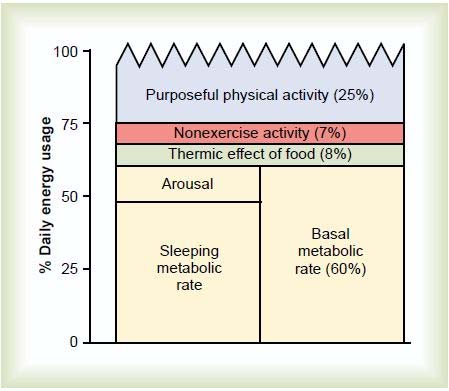
\includegraphics[width=0.6\textwidth]{../images/BMR_1.jpg}
\caption{Percentage breakdown of daily energy usage}
\label{bmr}
\end{figure}

\subsection*{Respiratory Quotient and Respiratory Exchange Ratio}
Because the amount of oxygen the cells consume and the amount of carbon dioxide they produce depends on the nutrients used for energy (i.e. enzymatic pathways for metabolizing carbohydrates, fats, and proteins generate different amounts of CO\textsubscript{2}), we can use these values to determine the fuel source.\\

Respiratory Quotient (RQ) defines the ratio of CO\textsubscript{2} produced to O\textsubscript{2} utilized by the cells and will vary depending on the substrate being metabolized (Table \ref{energy}), whereas Respiratory Exchange Ratio (RER) represents the ratio of CO\textsubscript{2} exhaled to O\textsubscript{2} consumed by the lungs. RER represents the average RQ of metabolism throughout the body under normal conditions.

\section*{Experimental Methods}
\subsection*{General Hardware and Software Setup}
\begin{enumerate}
	\item Gas Analysis System\begin{enumerate}
	\item Connect Gas-System2 to power supply and turn on to allow it to warm up for 5 min before calibration.
	\item Connect AFT7 tubing to inlet of Gas-System2 (Fig. \ref{aft}).\begin{figure}[h]
	\centering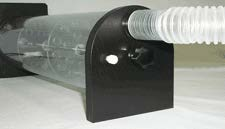
\includegraphics[width=0.5\textwidth]{../images/BMR_2.jpg}
		\caption{Inlet of Gas-System2 connected to AFT7 tubing}
		\label{aft}
		\end{figure}
	\end{enumerate}
	
	\item Assemble airflow accessories and connect them to the gas chamber. Keep in mind that some of these components might already be assembled (do not duplicate). See Fig. \ref{aft2} for a diagram.\begin{enumerate}
	\item Attach your disposable bacteriological filter (AFT1) to the inlet side of the airflow transducer (SS11LA).
	\item Connect AFT22 T-valve to opposite side of airflow transducer. Check that the arrows indicating airflow are pointing away from the airflow transducer.
	\item Connect AFT11C couplers to remaining two ports of T-valve.
	\item Use AFT11E (blue coupler) to connect AFT7 tubing to T-valve in the port opposite of SS11LA connection.
	\item Attach AFT6 calibration syringe to remaining port of T-valve.\begin{figure}[h]
	\centering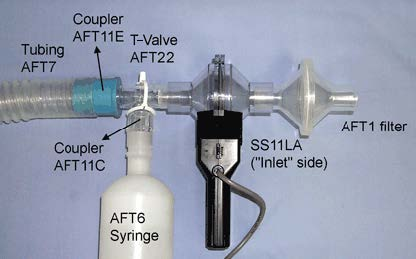
\includegraphics[width=0.5\textwidth]{../images/BMR_3.jpg}
		\caption{Schematic of airflow accessories connected to Gas-System2}
		\label{aft2}
		\end{figure}
	\end{enumerate}
	
	\item Connect SS11LA airflow transducer to channel 1.
	\item Connect O\textsubscript{2} output from Gas-System2 to channel 2.
	\item Connect CO\textsubscript{2} output from Gas-System2 to channel 3.
	\item Turn on MP3X.
\end{enumerate}

\subsection*{Calibration}
\begin{enumerate}
	\item Open file H19rer.gtl, which can be downloaded from the course website.
	\item Pump calibration syringe 15-20 times to flush Gas-System2 chamber with ambient air.
	\item Change acquisition length (Fig. \ref{acqlength}):\begin{enumerate}
	\item Select MP3X from the menu at the top of the screen.
	\item Choose Setup Acquisition.
	\item Make sure setup is set to \textit{Record} and \textit{Append}.
	\item Enter 100 samples/second under sample rate.
	\item Change the acquisition length to 50 minutes.
	\end{enumerate}
	
	\begin{figure}[h]
	\centering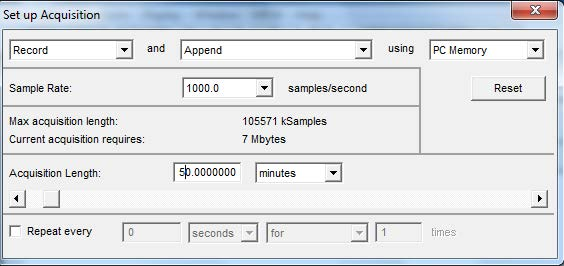
\includegraphics[width=0.5\textwidth]{../images/BMR_4.jpg}
		\caption{Setup acquisition window}
		\label{acqlength}
		\end{figure}
		
	\item Calibrate channels
	\begin{enumerate}
		\item Select MP3X from menu bar and select Setup Channels.
		\item Check all boxes for C6, VCO2.
		\item Uncheck all boxes for channel C7 (RER on MP30 and Vis on MP35).
		\item Calibrate airflow (channel 1)\begin{enumerate}
		\item Clock on wrench icon for channel 1.
		\item Click Scaling button to arrive to Change Scaling Parameters.
		\item Hold airflow transducer still and upright and press Cal1 button.
		\item Subtract 3000 from Ca1 value and enter as Cal2 input value field.
		\item Check Cal1 scale value is zero and Cal2 value is 10.
		\item Click OK twice to return to Setup Channels window.
		\end{enumerate}
		
		\item Calibrate O\textsubscript{2} (channel 2)\begin{enumerate}
			\item Click on wrench icon for channel 2.
			\item Click on Scaling button.
			\item Click on Cal2 button.
			\item Enter 20.93 as Cal2 scale value.
			\item Confirm that both Cal1 input value and Cal1 scale value are zero.
			\item Click OK twice to return to Setup Channels window.
		\end{enumerate}
		
		\item Calibrate CO\textsubscript{2} (channel 3)\begin{enumerate}
			\item Click on wrench icon for channel 3.
			\item Click on Scaling button.
			\item Click on Cal1 button.
			\item Enter value 0.04 as Cal1 scale value field.
			\item Add 10 to Cal1 input value and enter as Cal2 input value.
			\item Check Cal2 scale value is 1.04.
			\item Click OK twice to return to Setup Channels window.
		\end{enumerate}
		
		\item Click on wrench icon for C3 Vis (STPD).
		\item Update the formula to read C2*(0.898).
		\item Click OK to return to Setup Channels window.
		\item When done calibrating channels, press OK to return to principal window.
	\end{enumerate}
\end{enumerate}

\subsection{General Instructions}
\begin{enumerate}
	\item Before every trial, pump calibration syringe 15-20 times to flush the mixing chamber with ambient air.
	\item While recording, hold airflow apparatus very still, parallel to floor. Make sure to keep the airflow transducer handle perpendicular to floor.
	\item Begin every recording with inhalation and end with exhalation; this will prevent receiving O\textsubscript{2} inspiration values less than that of total expiration.
	\item Replace calibration syringe with AFT1 filter and AFT2 mouthpiece (Fig. \ref{aft3}).\begin{figure}[h]
	\centering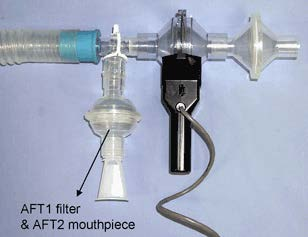
\includegraphics[width=0.5\textwidth]{../images/BMR_6.jpg}
		\caption{Schematic of airflow accessories with AFT1 filter and AFT2 mouthpiece}
		\label{aft3}
		\end{figure}
\end{enumerate}

The output from the BIOPAC Pro Software is summarized in Table \ref{abbreviation}.

\begin{table}[h]
	\centering
	\caption{BIOPAC Pro Software output}
	\begin{tabular}[h!]{p{0.5\textwidth}|p{0.15\textwidth}|p{0.15\textwidth}}
	\toprule
	Output & Abbreviation & Units\\
	\midrule
	Airflow through the pneumotachometer & Airflow & [L/sec]\\
	O\textsubscript{2} concentration in the mixing chamber & O2E (expired) & [volume \%]\\
	CO\textsubscript{2} concentration in the mixing chamber & CO2E (expired) & [volume \%]\\
	Volume of O\textsubscript{2} consumed at STP per 60 sec interval & VO2* & [L/min]\\
	Volume of CO\textsubscript{2} expired at STP per 60 sec interval & VCO2* & [L/min]\\
	\bottomrule
	\end{tabular}
	\label{abbreviation}
	\end{table}


\subsection*{Trial A: Basal/Abnormal Breathing Metabolic Measurements}
Trial A measures the BMR of a subject during normal breathing conditions and hyperventilation.
\begin{enumerate}
	\item Have the subject put on a nose clip.
	\item Start recording data by pressing the Start button located at the bottom left corner. Record a few seconds prior to breathing to ensure baselines are correct.
	\item Have the subject begin breathing normally through the mouthpiece for 2 minutes.
	\item Insert a marker in the recording and have the subject hyperventilate for 1 minute.
	\item Place a second marker and have the subject return to normal breathing. Collect 3 additional minutes of data.
	\item Stop recording and save your file with a unique name.
	\item Make sure that the data looks similar to Fig. \ref{baseline}. If it does, the subject should eat lunch.
	\begin{warn}
		If your data does not look similar to Fig. \ref{baseline}, rerun the test. Once the subject eats, this test cannot be redone, so obtain good data before continuing!
	\end{warn}
	
	\begin{figure}[h]
	\centering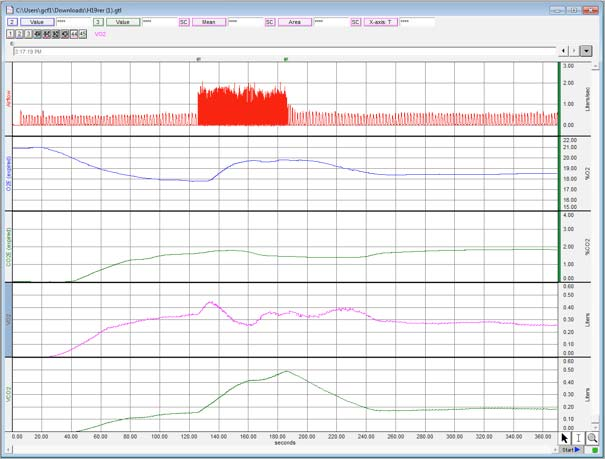
\includegraphics[width=0.6\textwidth]{../images/BMR_7.jpg}
		\caption{Expected data from Trial A}
		\label{baseline}
		\end{figure}

	\item Once finished, subject may eat lunch in preparation for Trial B.
	\item While the subject is eating, begin Trial C using a different subject.
\end{enumerate}

\subsection*{Trial B: Effects of Diet on BMR}
Trial B measures the metabolic rate of the subject after a meal.
\begin{enumerate}
	\item Wait approximately 30 minutes after the BMR subject's meal.
	\item If needed, repeat the calibration procedure described above.
	\item Use the calibration syring to purge the mixing chamber with 10-20 pumps.
	\item Have the subject put on the nose clip.
	\item Start recording data by pressing the Start button located at bottom left corner. Record a few seconds prior to breathing to ensure baselines are correct.
	\item Collect breathing data for 3 minutes.
	\item Stop recording and save your file.
\end{enumerate}

\subsection*{Trial C: Effects of Exercise on Metabolic Rate}
Trial C measures the metabolic rate and respiratory exchange ratio before and after exercise.
\begin{enumerate}
	\item If needed, repeat the calibration procedure described above.
	\item Use the calibration syringe to purge the mixing chamber with 10-20 pumps.
	\item This trial should be performed by a different subject that the subject from Trials A and B.
	\item Replace the inlet bacterial filter and mouthpiece at the T-valve. Do not replace the other filter at the air inlet.
	\item Have a new subject put on a nose clip and record 2 minutes of normal breathing data.
	\item Place a marker and stop recording.
	\item Flush the gas chamber with 15-20 pumps.
	\item Have the subject perform 5 minutes of aerobic exercise.
	\item Immediately after exercise, replace the nose clip and begin recording data from your subject.
	\item Record a few seconds without breathing to verify baseline gas values, then collect 6 minutes of breathing data.
	\item Stop data collection and save your file.
\end{enumerate}

\section*{Data Analysis}
Use the following values, if necessary:\begin{itemize}
	\item Ambient air composition by volume: 20.93\% O\textsubscript{2}, 0.04\% CO\textsubscript{2}, 79.03\% N\textsubscript{2}
	\item Vapor pressure of water is 22.4 mmHg and 75\degree F and 47.07 mmHg at 98.6\degree F
\end{itemize}

\begin{enumerate}
	\item Use data collected during Trial A. After equilibrium is reached in the mixing chamber (O\textsubscript{2} and CO\textsubscript{2} traces are stable and flat), report the metabolic rate (MR) and RER in the table in the handout using the following relationships:
	\begin{equation}
		MR\ [kcal/m^2/hr] \frac{}{Body\ Surface\ Area\ [m^2]}
	\end{equation}
\end{enumerate}

\end{document}
